\documentclass{slide}

% \usepackage{pgfpages}
% \setbeameroption{show notes on second screen}

\title{Distributed Computing III}
\subtitle{\textit{Murphy was an optimist} \newline \newline   % O'Toole's Commentary
CSSE6400}

\author{Richard Thomas}
\date{\week{10}}

\begin{document}

\maketitle

\questionanswer{What communication faults may occur?}{
    \begin{itemize}[<+(1)->]
        \item Message not delivered
        \item Message delayed
        \item Receiver failed
        \item Receiver busy
        \item Reply not received
        \item Reply delayed
    \end{itemize}
}
\note[itemize]{
    \item Lost in transit
    \item Network delay or receiver overloaded, but message will be processed later
    \item Receiver software has crashed or node has died
    \item Receiver temporarily not replying (e.g. garbage collection has frozen other processes)
    \item Request was processed but reply lost in transit
    \item Reply will be received later
}

\questionanswer{How do we detect faults?}{
    \begin{itemize}[<+(1)->]
        \item No listener on port -- RST or FIN packet
        \item Process crashes -- Monitor report failure
        \item IP address not reachable -- unreachable packet
        \item Query switches
        \item Timeout
    \end{itemize}
}
\note[itemize]{
    \item Assumes node is running \& reachable. OS should close or refuse connection. Error packet may be lost in transit.
    \item Assumes node is running \& reachable. Most reliable.
    \item Router has to determine address is not reachable, which is no easier than for your application.
    \item Need permissions to do this. Will only have this in your own data centre.
    \item UDP reduces network transmission time guarantee -- does not perform retransmission
}

\questionanswer{What to do if fault is detected?}{
    \begin{itemize}
        \item Retry
        \item Restart
    \end{itemize}
}
\note[itemize]{
    \item How many retries? How often?
    \item Exponential backoff with jitter
    \item How long to wait to restart?
    \item Too long reduces responsiveness.
    \item Unacknowledged messages need to be sent to other nodes -- reducing performance.
    \item Too short may prematurely declare nodes dead.
    \item May lead to contention -- two nodes processing the same request.
    \item May lead to cascading failure -- load is sent to other nodes, slowing them down so they are then declared dead \dots.
}

\definition{Idempotency}{
    Repeating an operation does not change receiver's state.
}
\note[itemize]{
    \item Idempotent consumer pattern
    \item Tag messages with an ID, so repeated messages can be ignored
    \item Or, redo messages that do not change state (e.g. queries)
}

\begin{frame}{Byzantine Generals Problem}
    \begin{columns}[onlytextwidth,T]
      \column{30mm}
        \vspace{2mm}
        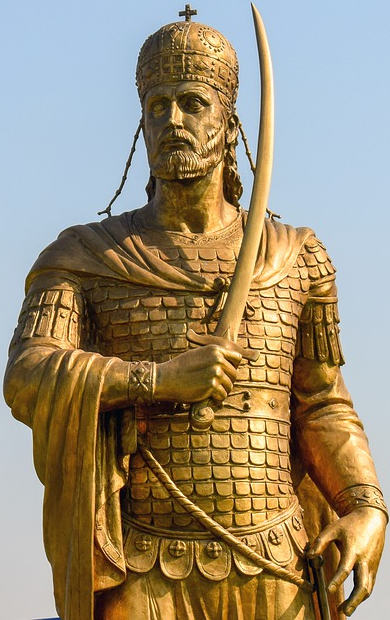
\includegraphics[width=30mm]{images/byzantine-general.jpg}  % From https://pixabay.com/photos/konstantinos-paleologos-emperor-4618859/

      \column{\dimexpr\linewidth-30mm-5mm}
        {\LARGE
        \begin{itemize}
            \item $n$ generals need to agree on plan
            \vspace{2mm}
            \item Can only communicate via messenger
            \item Messenger may be delayed or lost
            \vspace{2mm}
            \item Some generals are traitors
            \begin{itemize}
                \vspace{1mm}
                \Large\item Send dishonest messages
                \vspace{1mm}
                \Large\item Pretend to have not received message
            \end{itemize}
        \end{itemize}
        }
    \end{columns}
\end{frame}
\note[itemize]{
    \item Link analogy to Byzantine faults
    \item Mention idea of Byzantine fault-tolerant systems
    \item e.g. safety critical systems, blockchain, \dots
}

\definition{Poison Message}{
    A message that causes the receiver to fail.
}
\note[itemize]{
    \item Could literally cause the receiver to crash
    \item Often the receiver just cannot process the message and aborts processing
}

\begin{frame}{Poison Message}
    \begin{columns}[onlytextwidth,T]
      \column{\dimexpr\linewidth-30mm-5mm}
        {\LARGE
        \begin{itemize}
            \item Receiver can't process message
            \begin{itemize}
                \vspace{1mm}
                \Large\item Always fails
                \begin{itemize}
                    \large\item Not due to transient failure
                \end{itemize}
            \end{itemize}
            \vspace{2mm}
            \item Failed messages are retried
            \begin{itemize}
                \vspace{1mm}
                \Large\item Returned to front of queue
                \begin{itemize}
                    \large\item Preserve message order
                \end{itemize}
            \end{itemize}
            \vspace{2mm}
            \item Next receiver fails to process message
            \begin{itemize}
                \vspace{1mm}
                \Large\item Infinite loop
            \end{itemize}
            \vspace{2mm}
            \item Blocks sending of following messages
        \end{itemize}
        }

      \column{30mm}
        
\includegraphics[width=33mm]{images/poison-bottle.png}  % From https://pixabay.com/vectors/poison-bottle-toxic-chemistry-4662212/
    \end{columns}
\end{frame}
\note[itemize]{
    \item Elaborate on the error process and why it leads to the loop.
}

\questionanswer{What causes a message to be poisonous?}{
    \begin{itemize}
        \item<2-> Content is invalid
            \begin{itemize}
                \Large\item e.g. Invalid product id sent to purchasing service
                \vspace{1mm}
                \Large\item Error handling doesn't cater for error case
            \end{itemize}
            \vspace{2mm}
        \item<3-> System state is invalid
            \begin{itemize}
                \Large\item e.g. Add item to shopping cart that has been deleted
                \vspace{1mm}
                \Large\item Logic doesn't handle out of order messages
                \begin{itemize}
                    \large\item Insidious asynchronous faults
                \end{itemize}
            \end{itemize}
    \end{itemize}
}
\note[itemize]{
Invalid content may be
    \item corrupted data,
    \item old version of data structure,
    \item incorrect data, or
    \item malicious data.
}

\begin{frame}{Detecting Poison Messages}
    \vspace{1mm}
    {\LARGE
        Retry counter -- with limit
        \begin{itemize}
            \Large\item Where is counter stored?
            \begin{itemize}
                \large\item Memory -- What if server restarts?
                \vspace{1mm}
                \large\item DB -- Slow
                \vspace{2mm}
                \large\item Must ensure counter is reset, regardless of how message is handled
                \begin{itemize}
                    \item e.g. Message is manually deleted
                \end{itemize}
            \end{itemize}
        \end{itemize}
        \pause
        \vspace{3mm}
        Message service may have a timeout property
        \begin{itemize}
            \Large\item Message removed from queue
            \begin{itemize}
                \large\item Pending messages get older while waiting for poison message
                \vspace{1mm}
                \large\item Transient network faults may exceed timeout
            \end{itemize}
        \end{itemize}
    }
\end{frame}

\begin{frame}{Detecting Poison Messages}
    \vspace{1mm}
    {\LARGE
        Monitoring service
        \begin{itemize}
            \Large\item Trigger action if message stays at top of queue for too long
            \vspace{2mm}
            \Large\item Can check for queue errors
            \begin{itemize}
                \large\item No messages are being processed
                \vspace{1mm}
                \large\item Restart message service
            \end{itemize}
        \end{itemize}
    }
\end{frame}

\begin{frame}{Handling Poison Messages}
    \vspace{1mm}
    {\LARGE
        Discard message
        \begin{itemize}
            \Large\item System must not require guarantee of message delivery
            \Large\item Suitable when message processing speed is most important
        \end{itemize}
        \pause
        \vspace{3mm}
        Always retry
        \begin{itemize}
            \Large\item Requires mechanism to fix message
            \begin{itemize}
                \large\item Often requires manual intervention
            \end{itemize}
            \Large\item Suitable when message delivery is most important
            \Large\item Very long delays in processing
        \end{itemize}
    }
\end{frame}

\begin{frame}{Handling Poison Messages}
    \vspace{1mm}
    {\LARGE
        Dead-letter queue
        \begin{itemize}
            \Large\item Long transient failures result in adding many messages
            \begin{itemize}
                \large\item e.g. Network failure
            \end{itemize}
            \Large\item Requires manual monitoring and intervention
            \Large\item System must not require strict ordering of messages
            \Large\item Suitable when message processing speed is important
        \end{itemize}
    }
\end{frame}

\begin{frame}{Handling Poison Messages}
    \vspace{1mm}
    {\LARGE
        Retry queue
        \begin{itemize}
            \Large\item Transient failures also added
            \Large\item Use a previous strategy to deal with poison messages
            \Large\item System must not require strict ordering of messages
            \Large\item Suitable when message processing speed is very important
            \begin{itemize}
                \large\item Main queue is never blocked
                \large\item Receivers need to process from two message queues
            \end{itemize}
        \end{itemize}
    }
\end{frame}

\definition{Poison Pill Message}{
    Special message used to notify receiver it should no longer wait for messages.
}
\note{Emphasise that this is different to a poison message}

\questionanswer{Why use a poison pill message?}{
    Graceful shutdown of system.
}
\note[itemize]{
    \item Implementation is challenging with multiple producers and/or consumers
    \item It must be the last message received by all consumers
}

\questionanswer{How to order asynchronous messages?}{
    \begin{itemize}
        \item Timestamps?
        \begin{itemize}
            \vspace{1mm}
            \LARGE\item Can't keep clocks in sync
            \vspace{1mm}
            \LARGE\item Limited clock precision
        \end{itemize}
    \end{itemize}
}
\note[itemize]{
    \item Trying to sync with NTP is unreliable
    \item Network delays during sync
    \item Clock drift between syncs
    \item Finite precision -- two events may end up with the same timestamp, if they occur in quick succession
}

\point[Consistency]{
    \begin{description}
        \item[Eventual Consistency] weak guarantee
        \item[Linearisability] strong guarantee
        \item[Causal Ordering] strong guarantee
    \end{description}
}

\point[Linearisability]{
\begin{itemize}
    \item<1-> Once value is written, all reads see same value
    \begin{itemize}
        \LARGE\item<1-> Regardless of replica read from
    \end{itemize}
    \item<2-> Single-leader replication
    \begin{itemize}
        \LARGE\item<2-> Read from leader
        \LARGE\item<2-> Read from synchronous follower
    \end{itemize}
    \item<3-> Multi-leader replication can't be linearised
    \item<4-> Leaderless replication
    \begin{itemize}
        \LARGE\item<4-> Lock value on quorum before writing
    \end{itemize}
\end{itemize}
}
\note[itemize]{
    \item Abstraction over replicated database
    \item Used when uniqueness needs to be guaranteed
    \item e.g. Multiple withdrawals from an account
    \item SLR -- defeats most performance benefits
    \item Leaderless -- similar performance cost to SLR
}

\point[Causal Order]{
\begin{itemize}
    \item<1-> Order is based on causality
    \begin{itemize}
        \LARGE\item<1-> What event needs to happen before another
        \LARGE\item<1-> Allows concurrent events
    \end{itemize}
    \vspace{3mm}
    \item<2-> Single-leader replication
    \begin{itemize}
        \LARGE\item<2-> Record sequence number of writes in log
        \LARGE\item<2-> Followers read log to execute writes
    \end{itemize}
    \item<3-> Lamport timestamps
\end{itemize}
}
\note[itemize]{
    \item Linearisation defines a total order
    \item Causal ordering defines a partial order
    \item e.g. Git repo history with branching as causal order
    \item Not as strict as linearisability, so less performance cost
}

\image[trim=60 189 450 35,clip,height=\textheight]{../../notes/distributed3/diagrams/lamport-timestamp-seq.png}

\definition{Consensus}{
    A set of nodes in the system agree on some aspect of the system’s state.
}
\note{Abstraction to make it easier to reason about system state.}

\point[Consensus Properties]{
\begin{description}
    \item[Uniform Agreement] All nodes must agree on the decision
    \item[Integrity] Nodes can only vote once
    \item[Validity] Result must have been proposed by a node
    \item[Termination] Every node that doesn't crash must decide
\end{description}
}
\note[itemize]{
    \item Uniform agreement and integrity are key
    \item Validity avoids nonsensical solutions (e.g. always agreeing to a null decision)
    \item Termination enforces fault tolerance, it requires that progress is made towards a solution
}

\definition{Atomic Commit}{
    All nodes participating in a distributed transaction need to form consensus to complete the transaction.
}
\note{Based on transaction atomicity from ACID.}

\point[Two-Phase Commit]{
\begin{description}
    \item[Prepare] Confirm nodes can commit transaction
    \item[Commit] Finalise commit once consensus is reached
    \begin{itemize}
        \LARGE\item Abort if consensus can't be reached
    \end{itemize}
\end{description}
}

\image[trim=55 70 420 30,clip,height=\textheight]{../../notes/distributed3/diagrams/2phase-commit-seq.png}
\note[itemize]{
    \item Transaction ID used to track writes
    \item Prepare does all steps of a commit, aside from confirming it -- It cannot be revoked by participant
    \item Commit intent is recorded in log before sending to participants
    \item Even if a particiant fails, commit can proceed when it recovers
    \item Comment on performance costs
}

\end{document}